%%% Choose between 16:9 and 4:3 format by commenting out/uncommenting one of the following lines:
\documentclass[aspectratio=169]{beamer} % 16:9
% \documentclass{beamer} % 4:3

%=========================================================================================================================

\usepackage{lmodern}            % Latin Modern provides bold-italic shapes that cmss lacks
\usepackage[english]{babel}     % English language
\usepackage[latin1]{inputenc}   % Input encoding
\usepackage{tikz}               % For creating graphics
\usetikzlibrary{positioning, arrows.meta}
\usepackage{forest}             % For the taxonomy tree figure
\usepackage{url}                % For including urls
\usepackage{tabularx}           % For better tables
\usepackage{amsmath}            % Math environments
\usepackage{amsfonts}           % Math fonts
\usepackage{amssymb}            % Math symbols
\usepackage{acronym}            % Acronym management
\usepackage{booktabs}           % Professional table rules
\usepackage{listings}           % ASP code listings, matching thesis \S5
\lstset{
    basicstyle=\scriptsize\ttfamily,
    keywordstyle=\bfseries,
    commentstyle=\itshape\color{gray},
    breaklines=true,
    columns=fullflexible,
    keepspaces=true,
}
\lstdefinestyle{asp}{
    language={},
    alsoletter={\#,_},
    morekeywords={not, true, false, \#show, \#const, \#minimize, \#maximize},
    keywordstyle=\bfseries,
    morecomment=[l]{\%},
}
\usepackage{hyperref}           % Hyperlinks for backup slides
\hypersetup{hidelinks}

\usetheme{aig}                  % Set beamer theme

%=========================================================================================================================
\title{Inconsistency Measurement \\for Classical Planning Problems}
\subtitle{Master's Thesis Defense}

% if meta.tex does not exist, use default values
\InputIfFileExists{../meta.tex}{}{
    \newcommand{\authorname}{Erika Mustermann}
    \newcommand{\authname}{E. Mustermann}
}
\author[\authname]{\authorname}
\institute{Artificial Intelligence Group,\\
University of Hagen, Germany}
\date{July 1, 2026}
%========================================================================
\logo{\includegraphics[width=3cm]{figures/logoaig2025_transparent.png}}
%========================================================================

% Footer cite helper
\newcommand{\sectioncite}[1]{\hfill {\scriptsize \textcolor{gray}{#1}}}
% Footer cite with a hyperlink to a backup frame.
\newcommand{\sectioncitebk}[2]{\hfill {\scriptsize \textcolor{gray}{\hyperlink{#1}{[backup]}\quad #2}}}
\newcommand{\sectioncitebkk}[3]{\hfill {\scriptsize \textcolor{gray}{\hyperlink{#1}{[backup]}\quad\hyperlink{#2}{[backup]}\quad #3}}}

\begin{document}

\begin{frame}
    \titlepage
\end{frame}
\nologo

\begin{frame}{Overview}
    \tableofcontents
\end{frame}

%======================================
% MAIN DECK
%======================================

\section{Motivation}

% BUDGET: ~75s
\begin{frame}{Motivation}
    \begin{exampleblock}{A rover mission}
        A Mars rover carries five mission goals, among them sample the soil, image in two directions, map the surface, and reach orbit. No plan achieves all five, so the planner returns \textbf{Unsolvable}. Which goals fail, and how severe is each conflict?
    \end{exampleblock}

    \begin{alertblock}{The diagnostic gap}
        \begin{itemize}
            \item Planners give a binary answer, no further information about severity or structure
            \item Dead-state certificates [Eriksson et al., 2018] confirm unsolvability
            \item Excuses [G\"obelbecker et al., 2010] prescribe a repair
            \item None quantify how inconsistent the instance is
        \end{itemize}
    \end{alertblock}
    \sectioncite{Thesis \S1, \S3}
\end{frame}

\section{Problem and research questions}

% BUDGET: ~60s
\begin{frame}{Can inconsistency measurement explain planning failures?}
    \vfill
    \begin{block}{Central research question}
        \large
        How can inconsistency measures from propositional logic be meaningfully adapted to classical planning to provide diagnostic value for unsolvable planning problems?
    \end{block}
    \vfill
    \sectioncite{Thesis \S1.2}
\end{frame}

% BUDGET: ~60s
\begin{frame}{Adapt the measures, implement them, evaluate them}
    \begin{block}{RQ1\quad Theoretical adaptation}
        Which classical inconsistency measures adapt to planning, and which postulates carry over?
    \end{block}
    \begin{block}{RQ2\quad Implementation}
        How to compute the adapted measures efficiently using \ac{ASP}?
    \end{block}
    \begin{block}{RQ3\quad Practical evaluation}
        Do the adapted measures provide diagnostic value on real unsolvable benchmarks?
    \end{block}
    \sectioncite{Thesis \S1.2}
\end{frame}

\section{Foundations}

% BUDGET: ~60s
\begin{frame}{Inconsistency measure $\mathcal{I}(K)$}
    \begin{block}{Inconsistency measure $\mathcal{I} : \mathbb{K} \to \mathbb{R}_{\geq 0}$ [Thimm, 2019]}
        \begin{itemize}
            \item Higher value means more inconsistency, $\mathcal{I}(K) = 0$ iff $K$ consistent
            \item Rationality postulates such as Monotonicity and Free Formula Independence pin down sensible measures
            \item Contension $\mathcal{I}_c$ [Grant and Hunter, 2011] counts the atoms it must assign the truth value $B$, both true and false
        \end{itemize}
    \end{block}

    \begin{exampleblock}{Contension $\mathcal{I}_c$}
        $K = \{a \land b,\ \neg a,\ \neg b\}$ forces $a$ and $b$ to $B$, so $\mathcal{I}_c(K) = 2$.
    \end{exampleblock}
    \sectioncite{Thesis \S2.1}
\end{frame}

% BUDGET: ~60s
\begin{frame}{Classical planning}
    \small A PDDL Domain and Problem translate to a STRIPS tuple $\Pi = \langle P, O, I, G \rangle$.

    \begin{block}{STRIPS notation $\Pi = \langle P, O, I, G \rangle$ [Bylander 1994]}
        \footnotesize
        \begin{itemize}
            \item $P$ propositions, $O$ operators, $I \subseteq P$ initial state, $G \subseteq P$ goal
            \item Each operator $o = \langle \text{precond}(o), \text{add}(o), \text{delete}(o) \rangle$
            \item Plan is an applicable operator sequence from $I$ reaching a state $\supseteq G$. Unsolvable means none exists
        \end{itemize}
    \end{block}
    \begin{columns}[T]
        \begin{column}{0.6\textwidth}
            \begin{exampleblock}{Rover Mission, the drill subproblem}
                \footnotesize
                $P = \{\text{arm\_deployed},\ \text{drill\_bit},\ \text{hole\_drilled},\ \text{soil\_sampled}\}$ \\[2pt]
                $O = \{\ \text{drill} = \langle \{\text{arm\_deployed}, \text{drill\_bit}\},\ \{\text{hole\_drilled}\},\ \emptyset \rangle,$ \\[1pt]
                $\hphantom{O = \{\ } \text{sample} = \langle \{\text{hole\_drilled}\},\ \{\text{soil\_sampled}\},\ \emptyset \rangle\ \}$ \\[2pt]
                $I = \{\text{arm\_deployed}\}, \qquad G = \{\text{soil\_sampled}\}$
            \end{exampleblock}
        \end{column}
        \begin{column}{0.4\textwidth}
            \vspace*{-0.5em}
            \centering
            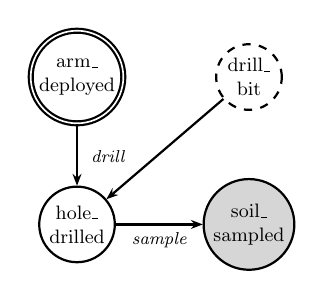
\begin{tikzpicture}[
        scale=0.78, transform shape,
        prop/.style={circle, draw, thick, font=\small, align=center, inner sep=1.5pt},
        missing/.style={prop, dashed},
        initial/.style={prop, double},
        goal/.style={prop, fill=black!16},
        oplbl/.style={font=\footnotesize\itshape},
        >={Stealth[length=1.5mm]},
    ]
    \node[initial] (arm)      at (0, 0)      {arm\_\\deployed};
    \node[missing] (drillbit) at (2.8, 0)    {drill\_\\bit};
    \node[prop]    (hole)     at (0, -2.4)   {hole\_\\drilled};
    \node[goal]    (soil)     at (2.8, -2.4) {soil\_\\sampled};
    \draw[->, thick] (arm)      -- (hole);
    \draw[->, thick] (drillbit) -- (hole);
    \node[oplbl] at (0.5, -1.3) {drill};
    \draw[->, thick] (hole) -- node[oplbl, below] {sample} (soil);
\end{tikzpicture}

        \end{column}
    \end{columns}

    \sectioncite{Thesis \S2.2}
\end{frame}

% BUDGET: ~60s
\begin{frame}{Answer Set Programming (ASP)}
    \begin{block}{Execution traces and reasoning modes}
        \begin{itemize}
            \item Each answer set of the encoding is one execution trace, a state sequence from $I$
            \item Brave reasoning unions the answer sets, an atom holds if some trace produces it
            \item Cautious reasoning intersects them, an atom holds only if every trace produces it [Eiter and Gottlob, 1995]
        \end{itemize}
    \end{block}

    \begin{exampleblock}{Brave and cautious over two traces}
        Trace 1 makes $\{a, b\}$ reachable, trace 2 makes $\{a, c\}$ reachable. \\[2pt]
        $\text{BRAVE} = \{a, b, c\}$ reachable by some trace, \quad $\text{CAUTIOUS} = \{a\}$ by every trace.
    \end{exampleblock}

    \sectioncite{Thesis \S2.4}
\end{frame}

\section{Taxonomy and design}

% BUDGET: ~60s
\begin{frame}{A taxonomy of unsolvability guides the measure design}
    \begin{center}
    \scalebox{0.68}{%
        \begin{forest}
            for tree={
                    rectangle, draw, rounded corners, thick,
                    align=center, font=\footnotesize,
                    minimum height=0.5cm,
                    inner sep=4pt,
                    l sep=3mm, s sep=2.5mm,
                    edge={thick},
                },
            inscope/.style={fill=black!16},
            where level=1{minimum width=2.9cm}{},
            where level=2{minimum width=2.4cm}{},
                [Unsolvable Planning\\Problems, minimum width=3.0cm, calign=child, calign child=2
                        [{Category 1:\\Operator-Induced\\Goal Conflicts}, inscope, tier=category
                        ]
                        [{Category 2:\\Dependency and\\Effect Structure}, inscope, tier=category, calign=child, calign child=2
                                [{2a: Missing\\producers}, inscope, thin
                                ]
                                [{2b: Circular\\dependencies}, thin
                                ]
                                [{2c: Action-based\\exclusions}, inscope, thin
                                ]
                        ]
                        [{Category 3:\\Resource\\Constraints}, tier=category
                        ]
                ]
        \end{forest}}

    \vspace{0.3em}
    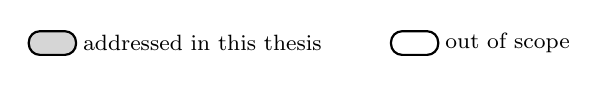
\begin{tikzpicture}[font=\footnotesize]
        \node[rectangle, draw, rounded corners, thick, fill=black!16,
            minimum width=0.6cm, minimum height=0.3cm] (in) at (0,0) {};
        \node[anchor=west, inner sep=2pt] at (in.east) {addressed in this thesis};
        \node[rectangle, draw, rounded corners, thick,
            minimum width=0.6cm, minimum height=0.3cm] (out) at (4.6,0) {};
        \node[anchor=west, inner sep=2pt] at (out.east) {out of scope};
    \end{tikzpicture}
\end{center}


    \begin{block}{Scope and overlap}
        \begin{itemize}
            \item $\mathcal{I}_{\text{MX}}$ for Category 1, $\mathcal{I}_{\text{GS}}$ for 2c, $\mathcal{I}_{\text{UR}}$ for unreachability across Category 2
            \item Dedicated 2b diagnosis needs graph analysis, Category 3 needs numeric fluents
            \item Categories overlap rather than partition, one problem may exhibit several
        \end{itemize}
    \end{block}

    \sectioncitebk{bk:overlap}{Thesis \S4.1}
\end{frame}

\section{Three diagnostic profiles}

% BUDGET: ~90s
\begin{frame}{Every profile pairs a goal-level count with a structural count}
    \begin{exampleblock}{Diagnostic profile shape}
        \[
            \mathcal{I}(\Pi, h) = (\mathcal{I}^{\text{scope}}(\Pi, h),\ \mathcal{I}^{\text{struct}}(\Pi, h))
        \]
    \end{exampleblock}

    \begin{block}{Two components, one parameter}
        \begin{itemize}
            \item Scope counts the affected goal propositions, structure the conflict artifacts beneath them
            \item Horizon $h \in \mathbb{N}$ bounds the reachability behind both counts
            \item Three measures share this shape, the Unreachability Profile $\mathcal{I}_{\text{UR}}$, the Goal Mutex Profile $\mathcal{I}_{\text{MX}}$, and the Goal Sequencing Conflict Profile $\mathcal{I}_{\text{GS}}$
        \end{itemize}
    \end{block}

    \sectioncitebk{bk:normalization}{Thesis \S4.4, \S4.6}
\end{frame}

% BUDGET: ~60s
\begin{frame}{$\mathcal{I}_{\text{UR}}$ counts goals the horizon never reaches}
    A goal proposition is unreachable when no state within horizon $h$ contains it. The scope variant counts these blocked goals, the structure variant counts every unreachable proposition, and the gap between them is the depth of the broken dependency chain.

    \begin{block}{Definition at horizon $h$}
        \begin{align*}
            \mathcal{I}^{\text{scope}}_{\text{UR}}(\Pi, h)  & = |\{g \in G \mid \nexists s \in S^h_{\text{reach}} : g \in s\}| \\
            \mathcal{I}^{\text{struct}}_{\text{UR}}(\Pi, h) & = |\{p \in P \mid \nexists s \in S^h_{\text{reach}} : p \in s\}|
        \end{align*}
    \end{block}

    \sectioncitebk{bk:bank-vault}{Thesis \S4.4.3}
\end{frame}

% BUDGET: ~60s
\begin{frame}{$\mathcal{I}_{\text{MX}}$ counts goals that never coexist}
    Two goals are mutex at horizon $h$, written $\text{mutex}_h(g_1, g_2)$, when each is reachable on its own but no reachable state holds both. The scope variant counts the goals caught in some mutex, the structure variant counts the unordered pairs.

    \begin{block}{Definition at horizon $h$}
        \begin{align*}
            \mathcal{I}^{\text{scope}}_{\text{MX}}(\Pi, h)  & = |\{g \in G \mid \exists g' \in G,\ g \neq g' : \text{mutex}_h(g, g')\}|          \\
            \mathcal{I}^{\text{struct}}_{\text{MX}}(\Pi, h) & = |\{\{g_1, g_2\} \mid g_1, g_2 \in G,\ g_1 \neq g_2,\ \text{mutex}_h(g_1, g_2)\}|
        \end{align*}
    \end{block}

    \sectioncite{Thesis \S4.4.4}
\end{frame}

% BUDGET: ~60s
\begin{frame}{$\mathcal{I}_{\text{GS}}$ counts goals blocked in one direction}
    An ordered pair $(g_1, g_2)$ is a sequencing conflict at horizon $h$, written $\text{sc}_h(g_1, g_2)$, when both goals are reachable yet no trace $\sigma_0, \ldots, \sigma_k$ with $k \leq h$ achieves $g_1$ and then $g_2$. The scope variant counts the goals involved, the structure variant counts the ordered pairs, so the blocking direction is preserved.

    \begin{block}{Definition at horizon $h$}
        \begin{align*}
            \mathcal{I}^{\text{scope}}_{\text{GS}}(\Pi, h)  & = |\{g \in G \mid \exists g' \in G : \text{sc}_h(g, g') \text{ or } \text{sc}_h(g', g)\}| \\
            \mathcal{I}^{\text{struct}}_{\text{GS}}(\Pi, h) & = |\{(g_1, g_2) \mid g_1, g_2 \in G,\ g_1 \neq g_2,\ \text{sc}_h(g_1, g_2)\}|
        \end{align*}
    \end{block}

    \sectioncitebk{bk:trust-travel}{Thesis \S4.4.5}
\end{frame}

% BUDGET: ~75s
\begin{frame}{One problem, three diagnoses}
    The same Rover Mission, now read by the three measures at convergence.

    \begin{exampleblock}{Rover Mission profile}
        \[
            (\mathcal{I}_{\text{UR}},\ \mathcal{I}_{\text{MX}},\ \mathcal{I}_{\text{GS}}) = ((1, 3),\ (4, 2),\ (2, 1))
        \]
    \end{exampleblock}

    \begin{block}{Each measure isolates one flaw}
        \begin{itemize}
            \item $\mathcal{I}_{\text{UR}} = (1, 3)$, the drill chain, one blocked goal over three unreachable propositions
            \item $\mathcal{I}_{\text{MX}} = (4, 2)$, two mutex pairs, the dish and the surface-orbit conflict
            \item $\mathcal{I}_{\text{GS}} = (2, 1)$, only the surface-orbit pair, the reversible dish has no direction
        \end{itemize}
    \end{block}

    {\small $\mathcal{I}_{\text{GS}}$ refines $\mathcal{I}_{\text{MX}}$ by direction, $\mathcal{I}_{\text{UR}}$ is orthogonal, so the three are complementary.}

    \sectioncitebkk{bk:signatures}{bk:seq-implies-mx}{Constructed running example}
\end{frame}

\section{Postulates and complexity}

% BUDGET: ~90s
\begin{frame}{Postulates for planning-adapted inconsistency measures}
    \begin{block}{Three planning-adapted postulates}
        \begin{itemize}
            \item Planning Consistency, $\mathcal{I}(\Pi, h) = 0$ iff $\Pi$ solvable at sufficient $h$
            \item Operator Monotonicity, more operators open new paths and can only lower $\mathcal{I}$
            \item Goal Monotonicity, more goals add requirements and can only raise $\mathcal{I}$
        \end{itemize}
    \end{block}

    \begin{center}
        \footnotesize
        \begin{tabular}{l cc cc cc}
            \toprule
                                  & \multicolumn{2}{c}{$\mathcal{I}_{\text{UR}}$} & \multicolumn{2}{c}{$\mathcal{I}_{\text{MX}}$} & \multicolumn{2}{c}{$\mathcal{I}_{\text{GS}}$}                                              \\
            \cmidrule(lr){2-3}\cmidrule(lr){4-5}\cmidrule(lr){6-7}
            Postulate             & scope                                         & struct                                        & scope                                         & struct       & scope        & struct       \\
            \midrule
            Planning Consistency  & $\times$                                      & $\times$                                      & $\times$                                      & $\times$     & $\times$     & $\times$     \\
            Operator Monotonicity & $\checkmark$                                  & $\checkmark$                                  & $\times$                                      & $\times$     & $\times$     & $\times$     \\
            Goal Monotonicity     & $\checkmark$                                  & $\checkmark$                                  & $\checkmark$                                  & $\checkmark$ & $\checkmark$ & $\checkmark$ \\
            \bottomrule
        \end{tabular}
    \end{center}

    {\small No single measure satisfies Planning Consistency. Characterizing every failure needs multiple measures together.}

    \sectioncitebkk{bk:postulates}{bk:op-mono-ce}{Thesis \S4.5.1}
\end{frame}

% BUDGET: ~60s
\begin{frame}{Complexity of planning-adapted inconsistency measures}
    \begin{block}{Complexity}
        Every decision problem for $\mathcal{I}_{\text{UR}}, \mathcal{I}_{\text{MX}}, \mathcal{I}_{\text{GS}}$ is PSPACE-complete, the value problems lie in FPSPACE.
    \end{block}

    \begin{block}{Why}
        \begin{itemize}
            \item Each measure is reachability analysis over the state space
            \item Plan existence is already PSPACE-complete [Bylander, 1994], and PSPACE is closed under complement and polynomial composition
            \item So thresholds and counting cannot escape PSPACE, computing the profile costs no more than deciding solvability
        \end{itemize}
    \end{block}

    \sectioncitebkk{bk:pspace-proof}{bk:pspace-compare}{Thesis \S4.5.3}
\end{frame}

\section{Implementation}

% BUDGET: ~90s
\begin{frame}{Brave reasoning replaces exponential trace enumeration}
    \begin{center}
        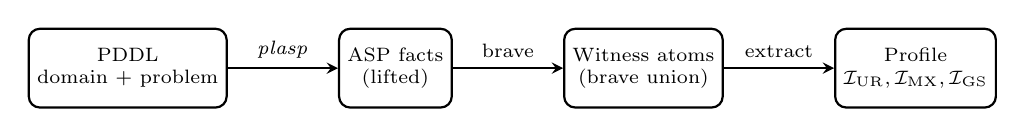
\begin{tikzpicture}[
                node distance=14mm,
                box/.style={rectangle, draw, rounded corners, thick, minimum height=10mm, align=center, inner sep=3pt, font=\scriptsize},
                arr/.style={-stealth, thick}
            ]
            \node[box]               (pddl) {PDDL\\ domain + problem};
            \node[box, right=of pddl] (asp) {ASP facts\\ (lifted)};
            \node[box, right=of asp]  (wit) {Witness atoms\\ (brave union)};
            \node[box, right=of wit] (prof) {Profile\\ $\mathcal{I}_{\text{UR}}, \mathcal{I}_{\text{MX}}, \mathcal{I}_{\text{GS}}$};
            \draw[arr] (pddl) -- node[above, font=\scriptsize]{\textit{plasp}} (asp);
            \draw[arr] (asp)  -- node[above, font=\scriptsize]{brave} (wit);
            \draw[arr] (wit)  -- node[above, font=\scriptsize]{extract} (prof);
        \end{tikzpicture}
    \end{center}

    \begin{block}{Key choice}
        \begin{itemize}
            \item \texttt{--enum-mode=brave} unions atoms true in at least one answer set
            \item Each answer set is one execution trace, and brave captures all without enumeration
            \item Witness atoms record whether goal pairs coexist or sequence
            \item Absence of a witness under brave proves no trace satisfies the condition
        \end{itemize}
    \end{block}

    \sectioncitebk{bk:asp-vs-sat}{Thesis \S5.1}
\end{frame}

% BUDGET: ~90s
\begin{frame}{Witness absence under brave reasoning is a universal proof}
    \begin{exampleblock}{Two witness atoms for goal pairs}
        \begin{itemize}
            \item \texttt{coexist\_witness($g_1$, $g_2$)} derived when some trace reaches a state with both goals
            \item \texttt{g2\_after\_g1\_witness($g_1$, $g_2$)} derived when some trace reaches $g_1$ then $g_2$
        \end{itemize}
    \end{exampleblock}

    \begin{block}{Brave gives the right semantics}
        \begin{itemize}
            \item $\text{BRAVE}(\Pi) = \bigcup_{S \in \text{AS}(\Pi)} S$, one answer set per trace
            \item Witness $\in \text{BRAVE}$ iff \emph{some} trace satisfies the condition; absence iff \emph{no} trace does, the mutex/sequencing definition
            \item Cautious uses $\bigcap$, requires \emph{every} trace to have the witness, wrong quantifier for non-existence claims
        \end{itemize}
    \end{block}

    \sectioncitebk{bk:asp-listing}{Thesis \S5.3.3}
\end{frame}

\section{Evaluation}

% BUDGET: ~90s
\begin{frame}{Evaluation setup}
    \begin{block}{Configuration}
        \begin{itemize}
            \item Horizon $h = 20$, time limit 120\,s, single Clingo thread
            \item Running on AMD Ryzen 5 5600X, 32\,GiB RAM, inside Docker
            \item Stack Python 3.12, Clingo 5.8.0, \textit{plasp} 3.1.1
        \end{itemize}
    \end{block}

    \begin{block}{Benchmark suites}
        \begin{itemize}
            \item IPC 2016 Unsolvability [Muise and Lipovetzky, 2016], 15 domains, 6 compatible
            \item Eriksson [Eriksson, 2019] adds \textit{3unsat} as the 7th compatible domain
            \item Two compatible solvable instances also run as sanity check
        \end{itemize}
    \end{block}

    \sectioncitebk{bk:horizon}{Thesis \S6.1}
\end{frame}

% BUDGET: ~90s
\begin{frame}{Evaluation results}
    \begin{exampleblock}{Coverage of the seven compatible domains}
        \centering\small
        \begin{tabular}{l c ccc c}
            \toprule
                                &                   & \multicolumn{3}{c}{instances with $\mathcal{I} > 0$} &                                         \\
            \cmidrule(lr){3-5}
            Domain              & OK / total        & UR                                                   & MX          & GS          & consistent  \\
            \midrule
            diagnosis           & 18 / 20           & 18                                                   & 2           & 2           & 0           \\
            3unsat              & 20 / 30           & 0                                                    & 0           & 0           & 20          \\
            bottleneck          & 12 / 25           & 0                                                    & 10          & 10          & 2           \\
            cave-diving         & 9 / 25            & 1                                                    & 0           & 0           & 8           \\
            pegsol-row5         & 3 / 15            & 3                                                    & 0           & 0           & 0           \\
            document-transfer   & 3 / 20            & 3                                                    & 0           & 0           & 0           \\
            chessboard-pebbling & 3 / 23            & 0                                                    & 3           & 3           & 0           \\
            \midrule
            \textbf{Total}      & \textbf{68 / 158} & \textbf{25}                                          & \textbf{15} & \textbf{15} & \textbf{30} \\
            \bottomrule
        \end{tabular}
    \end{exampleblock}

    {\footnotesize Timing each implementation phase shows that coverage is mostly compute-bound, solving dominates six of seven domains, grounding only the operator-heavy ones.}

    \sectioncitebkk{bk:per-domain}{bk:validation}{Thesis \S6.2}
\end{frame}

% BUDGET: ~60s
\begin{frame}{Selected case studies}
    \begin{columns}[t]
        \begin{column}{0.31\textwidth}
            \begin{exampleblock}{Scope grades severity}
                \textit{diagnosis} prob06 vs prob05 \\[4pt]
                $\mathcal{I}^{\text{scope}}_{\text{UR}} = 1$ vs $49$ \\[4pt]
                14\% vs 88\% of goals unreachable
            \end{exampleblock}
        \end{column}
        \begin{column}{0.31\textwidth}
            \begin{exampleblock}{Structure grades density}
                \textit{diagnosis} prob10 vs prob16 \\[4pt]
                $\mathcal{I}^{\text{struct}}_{\text{MX}} = 1$ vs $28$ \\[4pt]
                single pair vs clique, $28 = \binom{8}{2}$ proven bound
            \end{exampleblock}
        \end{column}
        \begin{column}{0.31\textwidth}
            \begin{exampleblock}{Pairwise blind spot}
                \textit{3unsat}, all measures $0$ \\[4pt]
                every goal pair coexists \\[4pt]
                no assignment satisfies all, pairwise misses the triple
            \end{exampleblock}
        \end{column}
    \end{columns}

    \vfill
    {\footnotesize The measures grade severity and density, and expose where pairwise analysis stops.}

    \sectioncitebk{bk:3unsat}{Thesis \S6.3}
\end{frame}

% BUDGET: ~75s
\begin{frame}{Soundness-coverage tradeoff}
    \begin{exampleblock}{\textit{diagnosis} prob10 across three horizons}
        \centering\footnotesize
        \begin{tabular}{rccc l}
            \toprule
            $h$ & $\mathcal{I}^{\text{scope}}_{\text{UR}}$ & $\mathcal{I}^{\text{scope}}_{\text{MX}}$ & $\mathcal{I}^{\text{scope}}_{\text{GS}}$ & Reading                             \\
            \midrule
            10  & 19                                       & 0                                        & 0                                        & conflicting goals not yet reachable \\
            20  & 14                                       & 2                                        & 2                                        & apparent mutex and sequencing       \\
            30  & 11                                       & 0                                        & 0                                        & longer trace resolves the conflict  \\
            \bottomrule
        \end{tabular}
    \end{exampleblock}

    \begin{block}{The tradeoff}
        \begin{itemize}
            \item Soundness side, unreachability falls monotonically, mutex and sequencing do not, so short horizons give false positives
            \item Coverage side, each time step grows the ground program, fewer instances complete
            \item $h = 20$ balances the two, no single optimum, no solvable instance reports a conflict
        \end{itemize}
    \end{block}

    \sectioncitebk{bk:horizon}{Thesis \S6.4}
\end{frame}

\section{Conclusion}

% BUDGET: ~90s
\begin{frame}{Conclusion}
    \begin{columns}[t]
        \begin{column}{0.48\textwidth}
            \begin{block}{Contributions}
                \begin{itemize}
                    \item RQ1, three planning-native profiles $\mathcal{I}_{\text{UR}}$, $\mathcal{I}_{\text{MX}}$, $\mathcal{I}_{\text{GS}}$
                    \item RQ2, ASP brave-reasoning pipeline where a missing witness atom proves unsatisfiability
                    \item RQ3, 68 of 158 instances diagnosed, distinguishing structurally different unsolvability categories
                \end{itemize}
            \end{block}
        \end{column}
        \begin{column}{0.48\textwidth}
            \begin{block}{Limitations and future work}
                \begin{itemize}
                    \item Grounding bottleneck, 57\% time out \\ $\to$ lifted or MaxSAT encodings
                    \item Horizon dependence, no sufficient $h$ \\ $\to$ adaptive iterative deepening
                    \item Pairwise blind spot on $k$-tuples \\ $\to$ extend mutex and sequencing
                    \item Diagnosis only, not repair \\ $\to$ minimal-modification repair
                \end{itemize}
            \end{block}
        \end{column}
    \end{columns}

    \vfill
    \only<2->{\hfill\textit{Thank you!}}
\end{frame}


%======================================
% BACKUP DECK
%======================================

\appendix

\section*{Backup}

\begin{frame}[noframenumbering,plain]
    \vfill
    \begin{center}
        {\Huge\bfseries Backup slides}\\[1em]
        {\large Reachability, proofs, postulates, performance, scenarios}
    \end{center}
    \vfill
\end{frame}

%========================================================================
% Limitations of a propositional encoding (Thesis \S4.2)
%========================================================================

\begin{frame}[noframenumbering]{Backup, a propositional encoding of the drill chain works\dots}
    \hypertarget{bk:naive-drill}{}
    To build a propositional encoding from a planning problem, use the following rules:
    \begin{itemize}
        \item Each goal becomes a fact
        \item Each produced proposition implies its operator's preconditions and the negation of its delete effects
        \item The closed-world assumption negates every proposition that no operator produces and that is absent from $I$
    \end{itemize}

    \begin{columns}[T]
        \begin{column}{0.6\textwidth}
            \begin{exampleblock}{Propositional Encoding $K_{\text{drill}}$}
                \footnotesize
                $K_{\text{drill}} = \{\ \text{soil\_sampled},$ \hfill {\scriptsize\textcolor{gray}{goal}} \\[2pt]
                $\hphantom{K_{\text{drill}} = \{\ } \text{soil\_sampled} \rightarrow \text{hole\_drilled},$ \hfill {\scriptsize\textcolor{gray}{sample precond.}} \\[2pt]
                $\hphantom{K_{\text{drill}} = \{\ } \text{hole\_drilled} \rightarrow \text{arm\_deployed} \land \text{drill\_bit},$ \hfill {\scriptsize\textcolor{gray}{drill precond.}} \\[2pt]
                $\hphantom{K_{\text{drill}} = \{\ } \neg \text{drill\_bit}\ \}$ \hfill {\scriptsize\textcolor{gray}{closed world assumption}} \\[4pt]
                $\mathcal{I}_c(K_{\text{drill}}) = 1$, forcing \textit{drill\_bit} to $B$
            \end{exampleblock}
        \end{column}
        \begin{column}{0.4\textwidth}
            \centering
            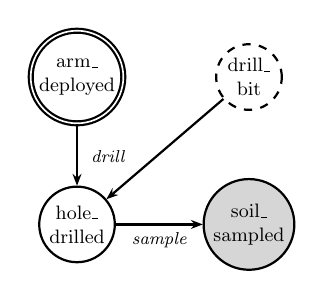
\begin{tikzpicture}[
        scale=0.78, transform shape,
        prop/.style={circle, draw, thick, font=\small, align=center, inner sep=1.5pt},
        missing/.style={prop, dashed},
        initial/.style={prop, double},
        goal/.style={prop, fill=black!16},
        oplbl/.style={font=\footnotesize\itshape},
        >={Stealth[length=1.5mm]},
    ]
    \node[initial] (arm)      at (0, 0)      {arm\_\\deployed};
    \node[missing] (drillbit) at (2.8, 0)    {drill\_\\bit};
    \node[prop]    (hole)     at (0, -2.4)   {hole\_\\drilled};
    \node[goal]    (soil)     at (2.8, -2.4) {soil\_\\sampled};
    \draw[->, thick] (arm)      -- (hole);
    \draw[->, thick] (drillbit) -- (hole);
    \node[oplbl] at (0.5, -1.3) {drill};
    \draw[->, thick] (hole) -- node[oplbl, below] {sample} (soil);
\end{tikzpicture}

        \end{column}
    \end{columns}

    \sectioncite{Thesis \S4.2}
\end{frame}

\begin{frame}[noframenumbering]{\dots\ but flattens every conflict to $\mathcal{I}_c = 1$}
    \hypertarget{bk:naive-flat}{}
    \begin{exampleblock}{$\mathcal{I}_c$ across three structurally distinct conflicts}
        \centering
        \begin{tabular}{lc}
            \toprule
            Planning failure                        & $\mathcal{I}_c$ \\
            \midrule
            Goal with no producer                   & $1$             \\
            Two goals that never hold together      & $1$             \\
            A goal that irreversibly blocks another & $1$             \\
            \bottomrule
        \end{tabular}
    \end{exampleblock}

    \begin{block}{Why the score is uninformative}
        \begin{itemize}
            \item $B$ absorbs each conflict at a single proposition, scoring a flat $1$
            \item Structural information is lost, so $\mathcal{I}_c$ cannot tell these failures apart
        \end{itemize}
    \end{block}

    \sectioncite{Thesis \S4.2}
\end{frame}

%========================================================================
% Taxonomy of unsolvable planning problems (Thesis \S4.1)
%========================================================================

\begin{frame}[noframenumbering]{Backup, the full taxonomy and what is in scope}
    \hypertarget{bk:taxonomy-tree}{}
    \begin{center}
    \scalebox{0.68}{%
        \begin{forest}
            for tree={
                    rectangle, draw, rounded corners, thick,
                    align=center, font=\footnotesize,
                    minimum height=0.5cm,
                    inner sep=4pt,
                    l sep=3mm, s sep=2.5mm,
                    edge={thick},
                },
            inscope/.style={fill=black!16},
            where level=1{minimum width=2.9cm}{},
            where level=2{minimum width=2.4cm}{},
                [Unsolvable Planning\\Problems, minimum width=3.0cm, calign=child, calign child=2
                        [{Category 1:\\Operator-Induced\\Goal Conflicts}, inscope, tier=category
                        ]
                        [{Category 2:\\Dependency and\\Effect Structure}, inscope, tier=category, calign=child, calign child=2
                                [{2a: Missing\\producers}, inscope, thin
                                ]
                                [{2b: Circular\\dependencies}, thin
                                ]
                                [{2c: Action-based\\exclusions}, inscope, thin
                                ]
                        ]
                        [{Category 3:\\Resource\\Constraints}, tier=category
                        ]
                ]
        \end{forest}}

    \vspace{0.3em}
    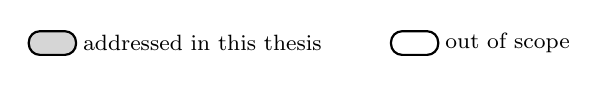
\begin{tikzpicture}[font=\footnotesize]
        \node[rectangle, draw, rounded corners, thick, fill=black!16,
            minimum width=0.6cm, minimum height=0.3cm] (in) at (0,0) {};
        \node[anchor=west, inner sep=2pt] at (in.east) {addressed in this thesis};
        \node[rectangle, draw, rounded corners, thick,
            minimum width=0.6cm, minimum height=0.3cm] (out) at (4.6,0) {};
        \node[anchor=west, inner sep=2pt] at (out.east) {out of scope};
    \end{tikzpicture}
\end{center}

    \begin{block}{Scope and overlap}
        \begin{itemize}
            \item State reachability is the common basis for Categories 1, 2a, and 2c
            \item Category 2b diagnosis needs graph analysis, Category 3 needs numeric fluents
            \item Categories overlap rather than partition, one problem may exhibit several types
        \end{itemize}
    \end{block}

    \sectioncite{Thesis \S4.1}
\end{frame}

%========================================================================
% Planning-native measures -- scenarios and normalization (Thesis \S4.3, \S4.4, \S4.6)
%========================================================================

\begin{frame}[noframenumbering]{Backup, reachable states and the horizon bound}
    \hypertarget{bk:reachability}{}
    \begin{block}{Reachable states}
        $S^0_{\text{reach}} = \{I\}$ \\[2pt]
        $S^{i+1}_{\text{reach}} = S^i_{\text{reach}} \cup \{\text{RESULT}(s, o) \mid s \in S^i_{\text{reach}},\ o \in O,\ \text{precond}(o) \subseteq s\}$
    \end{block}

    \begin{block}{Horizon bound}
        \begin{itemize}
            \item Ascending chain $S^0_{\text{reach}} \subseteq S^1_{\text{reach}} \subseteq \cdots$ converges at $h^* \leq 2^{|P|}$, each step only adds states
            \item $h^*$ is worst-case exponential, so the evaluation bounds it at $h = 20$
        \end{itemize}
    \end{block}

    \sectioncite{Thesis \S4.4.2}
\end{frame}

\begin{frame}[noframenumbering]{Backup, the isolated scenarios behind the running example}
    \hypertarget{bk:signatures}{}
    \begin{center}
        \scriptsize
        \begin{tabular}{l cc cc cc}
            \toprule
            Scenario         & \multicolumn{2}{c}{$\mathcal{I}_{\text{UR}}$} & \multicolumn{2}{c}{$\mathcal{I}_{\text{MX}}$} & \multicolumn{2}{c}{$\mathcal{I}_{\text{GS}}$}                           \\
            \cmidrule(lr){2-3}\cmidrule(lr){4-5}\cmidrule(lr){6-7}
                             & scope                                         & struct                                        & scope                                         & struct & scope & struct \\
            \midrule
            Locked Door      & 1                                             & 3                                             & 0                                             & 0      & 0     & 0      \\
            Bank Vault       & 1                                             & 7                                             & 0                                             & 0      & 0     & 0      \\
            Light Switch     & 0                                             & 0                                             & 2                                             & 1      & 0     & 0      \\
            Traffic Light    & 0                                             & 0                                             & 3                                             & 3      & 0     & 0      \\
            Trust and Travel & 0                                             & 0                                             & 2                                             & 1      & 2     & 1      \\
            Rival Alliances  & 0                                             & 0                                             & 2                                             & 1      & 2     & 2      \\
            \midrule
            Rover Mission    & 1                                             & 3                                             & 4                                             & 2      & 2     & 1      \\
            \bottomrule
        \end{tabular}
    \end{center}

    \begin{block}{The Rover Mission composes three canonical patterns}
        Drill chain $=$ Locked Door, dish toggle $=$ Light Switch, orbit chain $=$ Trust and Travel. The per-measure counts add to $(1, 3, 4, 2, 2, 1)$.
    \end{block}

    \sectioncite{Thesis \S4.3.4, \S4.4}
\end{frame}

\begin{frame}[noframenumbering]{Backup, absolute counts instead of normalized measures}
    \hypertarget{bk:normalization}{}
    \begin{exampleblock}{Relative measures exist [Besnard and Grant, 2020]}
        Dividing by $|G|$, $|P|$, or the maximal conflict count would yield percentage-style scores comparable across problem sizes.
    \end{exampleblock}

    \begin{block}{Why the profiles stay absolute}
        \begin{itemize}
            \item Severity is not proportional to size, 2 conflicting goals among 100 may be easier to repair than a complete clique on 3
            \item Every denominator choice encodes an assumption about problem structure
            \item Profiles carry relative information, scope against structure within each measure
            \item Future work could calibrate normalization against the IPC benchmark distribution
        \end{itemize}
    \end{block}

    \sectioncite{Thesis \S4.6.2}
\end{frame}

%========================================================================
% Postulates and complexity (Thesis \S4.5)
%========================================================================

\begin{frame}[noframenumbering]{Backup, postulate choice and the combined measure}
    \hypertarget{bk:postulates}{}
    \begin{block}{Why these three postulates}
        \begin{itemize}
            \item Classical postulates assume formula structure, planning has goals, operators, and states
            \item Adding operators can resolve conflicts, so Monotonicity reverses sign
            \item Modified postulates and the multi-measure approach follow the ASP precedent [Ulbricht et al., 2016]
        \end{itemize}
    \end{block}

    \sectioncite{Thesis \S4.5.1, \S6.3.6, \S7.4}
\end{frame}

\begin{frame}[noframenumbering]{Backup, adding an operator can raise $\mathcal{I}_{\text{MX}}$ and $\mathcal{I}_{\text{GS}}$}
    \hypertarget{bk:op-mono-ce}{}
    \begin{exampleblock}{One construction breaks both, $P = \{a, g_1, g_2\}$, $I = \{a\}$, $G = \{g_1, g_2\}$}
        \footnotesize
        Start with $O = \{\,\textit{reach\_g1} = \langle \{a\}, \{g_1\}, \{a\}\rangle\,\}$, then add $\textit{reach\_g2} = \langle \{a\}, \{g_2\}, \{a\}\rangle$.\\[2pt]
        \centering
        \begin{tabular}{lcc}
            \toprule
                                      & before add & after add \\
            \midrule
            $\mathcal{I}_{\text{MX}}$ & $(0, 0)$   & $(2, 1)$  \\
            $\mathcal{I}_{\text{GS}}$ & $(0, 0)$   & $(2, 2)$  \\
            \bottomrule
        \end{tabular}
    \end{exampleblock}

    \begin{block}{Why the value rises, and why $\mathcal{I}_{\text{UR}}$ is immune}
        \footnotesize
        \begin{itemize}
            \item Before, $g_2$ is unreachable, so no mutex pair and no sequencing conflict can form
            \item The added operator makes $g_2$ reachable but deletes $a$, which nothing re-adds, so no reachable state holds both goals
            \item This operator-induced mutex, with neither order achievable, raises $\mathcal{I}$, while $\mathcal{I}_{\text{UR}}$ only falls as $S^h_{\text{reach}}$ grows
        \end{itemize}
    \end{block}

    \sectioncite{Thesis \S4.5.1}
\end{frame}

\begin{frame}[noframenumbering]{Backup, sequencing implies mutex}
    \hypertarget{bk:seq-implies-mx}{}
    \begin{exampleblock}{Proposition}
        For any $\Pi$ and horizon $h$, if $(g_1, g_2)$ is a sequencing conflict with $g_2$ achievable, then $\{g_1, g_2\}$ is a mutex pair at horizon $h$.
    \end{exampleblock}

    \begin{block}{Proof sketch and counterexample}
        \begin{itemize}
            \item Sequencing makes both achievable, yet no trace has $g_1$ at $\sigma_i$, $g_2$ at $\sigma_j$, $i \leq j$
            \item The $i = j$ case is the mutex condition, which with achievability is the mutex definition
            \item On the Rover the sequencing pair $(\text{in\_orbit}, \text{mapped})$ is also one of the two mutex pairs, as the proposition predicts
            \item Converse fails on the dish toggle, $\{\text{aimed\_earth}, \text{aimed\_probe}\}$ is mutex yet reversible, so neither order is a sequencing conflict
        \end{itemize}
    \end{block}

    \sectioncite{Thesis \S4.5.2}
\end{frame}

\begin{frame}[noframenumbering]{Backup, PSPACE-completeness proof sketch}
    \hypertarget{bk:pspace-proof}{}
    \begin{block}{Membership of $\text{UPPER}_{\mathcal{I}_{\text{UR}}}$ in PSPACE}
        \footnotesize
        \begin{itemize}
            \item Guess an operator trace from $I$ in polynomial space, accept when $g$ appears
            \item NPSPACE $=$ PSPACE by Savitch, iterating over $|G|$ goals stays polynomial
        \end{itemize}
    \end{block}

    \begin{block}{Hardness via reduction from PlanSat}
        \footnotesize
        From $\Pi = \langle P, O, I, G \rangle$, build $\Pi' = \langle P \cup \{g^*\},\ O \cup \{o^*\},\ I,\ \{g^*\} \rangle$ with $o^* = \langle G, \{g^*\}, \emptyset \rangle$. Then $g^*$ is reachable iff $\Pi$ has a plan, so $\text{UPPER}_{\mathcal{I}_{\text{UR}}}$ at $k = 0$ decides PlanSat.
    \end{block}

    \begin{block}{Extends to MX, GS, and the other problems}
        \footnotesize
        \begin{itemize}
            \item For $\mathcal{I}_{\text{MX}}$ and $\mathcal{I}_{\text{GS}}$ a similar reduction makes the only path to $g_2$ delete $g_1$, so the pair is mutex or sequenced iff $\Pi$ is unsolvable
            \item LOWER is the complement of UPPER, EXACT checks both bounds, VALUE binary-searches UPPER, all staying in PSPACE or FPSPACE
        \end{itemize}
    \end{block}

    \sectioncite{Thesis \S4.5.3}
\end{frame}

\begin{frame}[noframenumbering]{Backup, PSPACE flattens the propositional multi-tier landscape}
    \hypertarget{bk:pspace-compare}{}
    \begin{exampleblock}{Decision-problem complexity, planning versus propositional $\mathcal{I}_c$}
        \centering
        \footnotesize
        \begin{tabular}{lll}
            \toprule
            Problem & Planning measures & Propositional $\mathcal{I}_c$ [Thimm and Wallner, 2016] \\
            \midrule
            UPPER   & PSPACE-complete   & NP-complete                                             \\
            LOWER   & PSPACE-complete   & coNP-complete                                           \\
            EXACT   & PSPACE-complete   & $D^p$-complete                                          \\
            VALUE   & FPSPACE           & FP$^{\text{NP}[\log n]}$-complete                       \\
            \bottomrule
        \end{tabular}
    \end{exampleblock}

    \begin{block}{Why the tiers collapse}
        \footnotesize
        \begin{itemize}
            \item Propositionally the base problem is satisfiability, NP-complete, so the measures stack into tiers above it
            \item For planning the base is PlanSat, already PSPACE-complete, a far larger ceiling
            \item PSPACE $=$ co-PSPACE collapses UPPER, LOWER, and EXACT, VALUE follows by polynomially many calls, so the gaps between measures vanish
        \end{itemize}
    \end{block}

    \sectioncite{Thesis \S4.5.3}
\end{frame}

%========================================================================
% Implementation (Thesis \S5)
%========================================================================

\begin{frame}[noframenumbering]{Backup, ASP reasoning modes, brave and cautious}
    \hypertarget{bk:asp-reasoning}{}
    \begin{block}{Execution traces and reasoning modes}
        \begin{itemize}
            \item Each answer set of the encoding is one execution trace, a state sequence from $I$
            \item Brave reasoning unions the answer sets, an atom holds if some trace produces it
            \item Cautious reasoning intersects them, an atom holds only if every trace produces it [Eiter and Gottlob, 1995]
        \end{itemize}
    \end{block}

    \begin{exampleblock}{Brave and cautious over two traces}
        Trace 1 makes $\{a, b\}$ reachable, trace 2 makes $\{a, c\}$ reachable. \\[2pt]
        $\text{BRAVE} = \{a, b, c\}$ reachable by some trace, \quad $\text{CAUTIOUS} = \{a\}$ by every trace.
    \end{exampleblock}

    \sectioncite{Thesis \S2.4}
\end{frame}

\begin{frame}[noframenumbering]{Backup, why ASP over SAT and MaxSAT}
    \hypertarget{bk:asp-vs-sat}{}
    \begin{block}{Reasons in favor of ASP}
        \begin{itemize}
            \item Default negation supports non-monotonic reasoning, matching reversed Operator Monotonicity
            \item Brave reasoning unions answer-set traces in one solver call, no manual enumeration
            \item ASP outperforms basic SAT encodings for inconsistency measures [Kuhlmann et al., 2025]
        \end{itemize}
    \end{block}

    \begin{block}{Trade-off acknowledged}
        Specialized MaxSAT beats ASP on classical formula-counting measures [Niskanen et al., 2023], and remains a future-work direction for scalability on planning-native measures.
    \end{block}

    \sectioncite{Thesis \S5, \S7.4}
\end{frame}

\begin{frame}[noframenumbering,fragile]{Backup, state-space exploration encoding}
    \hypertarget{bk:asp-listing}{}
    \begin{lstlisting}[style=asp]
time(0..horizon).
holds(P, 0) :- init(P).
% Applicability, positive and negative preconditions
neg_precond_violated(O, T) :- neg_precond(O, P), holds(P, T).
applicable(O, T) :- operator(O), time(T), T < horizon,
    not neg_precond_violated(O, T), holds(P, T) : precond(O, P).
% One operator per step, each choice a distinct trace
{ apply(O, T) : applicable(O, T) } 1 :- time(T), T < horizon.
% State transition with frame axiom
deleted(P, T) :- apply(O, T), delete(O, P).
holds(P, T+1) :- apply(O, T), add(O, P).
holds(P, T+1) :- holds(P, T), not deleted(P, T), time(T), T < horizon.
    \end{lstlisting}
    The choice rule branches into one answer set per execution trace. The frame axiom carries propositions forward unless an operator deletes them.

    \sectioncite{Thesis \S5.3.2}
\end{frame}

\begin{frame}[noframenumbering]{Backup, 80 automated tests verify the pipeline}
    \hypertarget{bk:validation}{}
    \begin{exampleblock}{Test suite}
        \begin{itemize}
            \item 80 tests across 8 categories, full suite runs in under one second
            \item 11 test scenarios match expected profiles exactly
            \item Categories cover scenarios, hierarchy, library API, end-to-end PDDL
        \end{itemize}
    \end{exampleblock}

    \begin{block}{Sample expected vs computed matches}
        \centering
        \scriptsize
        \begin{tabular}{lll}
            \toprule
            Category          & Scenario              & Profile              \\
            \midrule
            P1 Unreachability & Locked Door           & $(1, 3, 0, 0, 0, 0)$ \\
            P2 Mutex          & Traffic Light         & $(0, 0, 3, 3, 0, 0)$ \\
            P3 Sequencing     & Rival Alliances       & $(0, 0, 2, 1, 2, 2)$ \\
            Edge case         & Empty Goals           & $(0, 0, 0, 0, 0, 0)$ \\
            Edge case         & Negative Precondition & $(1, 1, 0, 0, 0, 0)$ \\
            \bottomrule
        \end{tabular}
    \end{block}

    \sectioncite{Thesis \S5.6}
\end{frame}

%========================================================================
% Evaluation (Thesis \S6)
%========================================================================

\begin{frame}[noframenumbering]{Backup, 3unsat and the $k$-tuple blind spot}
    \hypertarget{bk:3unsat}{}
    \begin{exampleblock}{Pairwise coexistence with no triple-satisfying state}
        \[
            G = \{g_1, g_2, g_3\}, \qquad
            S_{\text{reach}} \supseteq \{\{g_1, g_2\}, \{g_2, g_3\}, \{g_1, g_3\}\}
        \]
        Every pair is reachable together, yet no state satisfies all three.
    \end{exampleblock}

    \begin{block}{Consequence for the measures}
        \begin{itemize}
            \item All goals individually reachable, so $\mathcal{I}_{\text{UR}}(\Pi) = (0, 0)$
            \item No mutex pair exists in $S_{\text{reach}}$, so $\mathcal{I}_{\text{MX}}(\Pi) = (0, 0)$
            \item No ordered sequencing failure either, so $\mathcal{I}_{\text{GS}}(\Pi) = (0, 0)$
            \item All 20 completed \textit{3unsat} instances confirm this at every tested horizon
            \item Future work extends to $k$-tuple analysis for $|G| \geq 3$ failures
        \end{itemize}
    \end{block}

    \sectioncite{Thesis \S6.3.6, \S7.4}
\end{frame}


\end{document}
